\documentclass{article}
\usepackage[preprint,nonatbib]{neurips_2024}

\usepackage{pgfplots}

\usepackage{tikz}
\usepackage{amsmath}
\usepackage{amssymb}
\usetikzlibrary{positioning,arrows.meta,shapes.geometric}






\title{Exploring Contextual Flux in Large Language Models: A Novel Approach to Self-Modulating Semantic Networks}



\author{Henry Evidail \And Zachary Mountebank \And Alistair Hathersage \And Peter Stanhope \And Basil Ravenscroft \And Tobias Waddingham}


\begin{document}




\maketitle


\begin{abstract}
Self-modulating mechanisms introduce dynamic adaptation capabilities within language models through contextual realignment strategies that influence token embedding trajectories across extended sequences. Contextual Flux is explored as an approach to embedding modulation, integrating an auxiliary gating mechanism within the self-attention framework to dynamically adjust token representations based on evolving contextual dependencies. The empirical analysis evaluates entropy variations, latent space realignments, and coherence stability to assess the extent to which self-regulation enhances text generation consistency while preserving generative flexibility. Quantitative assessments suggest that embedding shifts contribute to more structured adaptation in long-form sequences, with measured reductions in redundant phrase repetitions and improvements in thematic retention. Variability in contextual weight computation affects modulation stability, leading to differing levels of adaptation across diverse linguistic structures. The computational demands introduced through real-time embedding reconfiguration are examined in relation to model scalability, emphasizing the need for optimization strategies in high-volume generative applications. The findings suggest that while adaptive embedding updates improve certain aspects of coherence, their impact remains contingent on model capacity and input complexity. 
\end{abstract}






\section{Introduction}
% Introduces the concept of Contextual Flux and the motivation behind exploring self-modulating semantic networks.

The evolution of natural language processing has been largely influenced by the development of Large Language Models (LLMs), which have demonstrated remarkable proficiency across a spectrum of linguistic tasks. Despite their impressive capabilities, LLMs often encounter challenges in maintaining contextual coherence during extended text generation. This limitation arises from their reliance on static learned representations, which can impede adaptability in dynamic discourse scenarios. Addressing this issue necessitates innovative approaches that enable models to adjust their semantic representations in real-time, thereby enhancing the fluidity and relevance of generated content. In response to this challenge, the present study introduces the concept of Contextual Flux, a novel mechanism designed to empower LLMs with the ability to autonomously modulate their internal semantic structures in alignment with evolving input contexts. This approach diverges from traditional memory-based architectures by embedding a self-regulating reconfiguration layer directly within the transformer attention heads. Through this integration, the model gains the capacity to dynamically recalibrate its attention mechanisms, facilitating a more nuanced understanding of context and promoting sustained thematic continuity over prolonged interactions.

The theoretical foundation of Contextual Flux is rooted in the dynamic adjustment of token embeddings, which are recalibrated based on their positional influence within the latent space. By implementing this mechanism, the model can achieve a more refined balance between preserving prior contextual information and integrating new inputs, thereby enhancing the overall coherence of generated narratives. This self-modulating capability is particularly advantageous in complex generative tasks, where the maintenance of contextual integrity is paramount. To empirically evaluate the efficacy of Contextual Flux, this study employs a recent open-source LLM as the experimental platform. The model is augmented with the proposed self-regulating reconfiguration layer, and its performance is assessed across a series of tasks designed to test contextual persistence and semantic adaptability. The experimental design emphasizes the autonomous functioning of the model, eliminating the need for explicit human intervention or external feedback mechanisms. This autonomy ensures that the observed enhancements in performance can be directly attributed to the intrinsic capabilities of the Contextual Flux mechanism.

The findings from this investigation are anticipated to contribute valuable insights into the development of more adaptable and contextually aware language models. By demonstrating the potential of self-modulating semantic networks, this research aims to pave the way for future advancements in LLM architectures that are capable of more fluid and contextually aligned text generation. The implications of such advancements extend to various applications, including conversational agents, content creation tools, and other AI-driven language technologies that demand a high degree of contextual sensitivity and coherence. The introduction of Contextual Flux represents a large step toward enhancing the adaptability of LLMs in dynamic discourse environments. By enabling models to autonomously adjust their semantic representations in response to evolving contexts, this approach addresses a critical limitation of existing architectures and opens new avenues for research and application in the field of natural language processing.




\section{Related Studies}
% Summarizes existing literature on latent representation shifts, attention-based memory mechanisms, and contextual adaptation in LLMs.

Research into Large Language Models (LLMs) has increasingly focused on mechanisms that enable more effective handling of extended dependencies, complex semantic structures, and evolving discourse patterns. The reliance on fixed learned representations has presented challenges in dynamically adjusting to contextual shifts, prompting investigations into various strategies aimed at enhancing adaptability without requiring external memory augmentation or human intervention. Recent advancements have explored mechanisms such as latent representation modulation, memory-based attention refinements, self-regulating embedding calculations, and dynamic token realignment techniques. A fundamental challenge in this domain has been ensuring that models can maintain coherence across longer sequences while minimizing loss of previously established semantic associations. While large progress has been made through architectural modifications and training paradigm shifts, the development of self-modulating contextual embedding shifts remains an area of ongoing investigation.

\subsection{Latent Representation Modulation}

Latent representation modulation has been a key area of study in improving the adaptability of LLMs in complex generative tasks. Investigations have demonstrated that dynamically altering latent representations through stochastic embedding transitions can provide a more flexible mechanism for adjusting token distributions in response to shifting input contexts \cite{kuse2024dynamic}. Instead of relying on static embeddings, techniques have been introduced that employ probabilistic modulation to refine token activation patterns based on surrounding contextual cues \cite{higginbotham2024prompting}. By implementing structured latent perturbations within transformer attention heads, models exhibited a more diverse range of sentence continuations, leading to greater robustness against repetitive phrase generation \cite{vitiello2024context}. Further analysis revealed that modulating token embedding trajectories led to improved generalization across diverse linguistic tasks without requiring additional external memory augmentation \cite{korbanov2024hierarchical}. This approach enabled models to allocate representational capacity more efficiently, reducing over-reliance on high-frequency token mappings while preserving semantic stability over extended text sequences \cite{harrow2024contextual}. Through latent structure realignment strategies, researchers demonstrated that self-adjusting token interactions reduced information loss in multi-turn text generation scenarios, thereby enhancing contextual retention across various domains \cite{ikaris2024context}. A comparative evaluation against conventional fixed-representation models indicated that self-modulating latent adjustments achieved improved coherence and structural fluency without necessitating modifications to transformer weight optimization protocols \cite{wench2024factored}.

\subsection{Attention-Based Memory Mechanisms}

Memory-integrated attention structures have been extensively explored to mitigate the contextual degradation observed in long-form text generation. The introduction of hierarchical attention gating mechanisms allowed for more refined control over how prior context was retained within successive decoding steps \cite{mahene2024automated}. A structured memory retention framework was developed in which long-range dependencies were selectively reinforced through self-regulating attention weight redistribution, reducing the tendency of LLMs to discard earlier contextual associations \cite{cakel2024daniel}. Empirical assessments highlighted that memory-conditioned attention adjustments largely lowered perplexity rates, suggesting improved predictive alignment in extended conversational tasks \cite{leonardi2024contextual}. It was observed that fine-tuned memory persistence configurations facilitated a smoother transition between discourse topics while preserving relevant thematic elements from preceding interactions \cite{bernar2024exploring}. Further experimentation demonstrated that attention reallocation techniques improved the model’s ability to generate logically structured responses that remained consistent over longer dialogue sessions \cite{harrington2024mitigating}. In addition, weight redistribution mechanisms provided adaptive weighting for tokens with stronger semantic relevance, leading to refined word selection strategies in open-ended generative tasks \cite{vulpescu2024optimized}.

\subsection{Contextual Embedding Adjustments}

Embedding modification strategies have been proposed to enhance the ability of LLMs to maintain coherence across evolving contexts. Techniques for real-time embedding shifts enabled models to adjust token-level representations based on their contribution to prior linguistic structures, thereby refining lexical prediction accuracy across diverse textual domains \cite{murph2024dynamic}. A comparative study of fixed versus adaptable embedding strategies showed that models employing self-regulating embedding realignment achieved more stable perplexity metrics and exhibited improved sentence continuity over long-form discourse generation \cite{embury2024dynamic}. By incorporating reinforcement-modulated embedding recalibration functions, it was demonstrated that models exhibited greater sensitivity to context-dependent linguistic variations, allowing for more refined token substitution behavior without explicit supervised intervention \cite{mcintosh2024inadequacy}. It was further established that embedding variance minimization strategies led to smoother sentence transitions, as models dynamically reweighted their latent representations based on inferred semantic relevance \cite{fa2024modality}. When tested across multilingual benchmarks, adaptable embedding mechanisms exhibited superior performance in language transfer tasks, indicating a stronger capacity for generalization beyond monolingual training data distributions \cite{giacomozzi2024innovative}. Contextual embedding adjustment frameworks also improved the ability of LLMs to handle ambiguous pronoun resolution challenges by maintaining latent referential consistency throughout extended narratives \cite{racus2024dynamic}. Additional experiments indicated that controlled embedding perturbations improved the model’s adaptability in response to minor input modifications, demonstrating resilience against adversarial text alterations \cite{ taillieu2024dynamic}.

\subsection{Dynamic Embedding Spaces}

Dynamic embedding spaces have been extensively examined as a mechanism for improving adaptability in token representation structures within LLMs. A probabilistic framework was introduced that allowed embeddings to shift dynamically based on input structure, effectively mitigating the tendency for models to exhibit excessive lexical repetition in constrained generative settings \cite{baronova2024dynamic}. It was observed that embedding space calculations that maintained continuity with prior token distributions enabled smoother linguistic transitions across variable-length sequences \cite{sawhai2024token}. Evaluations conducted on large-scale conversational datasets indicated that models with dynamically evolving embedding structures outperformed static-embedding configurations in preserving topic consistency over longer interaction windows \cite{ tokar2024contextual}. Controlled variation in token embedding space led to a marked decrease in mode collapse effects, where generative outputs otherwise displayed excessive reliance on a limited subset of high-frequency tokens \cite{chen2024dynamic}. The introduction of self-modulating positional embedding systems further enabled models to dynamically reweight token importance based on latent discourse patterns, improving sentence fluency and logical flow \cite{sasaki2024enhancing}. Additional refinements in dynamic embedding scaling mechanisms demonstrated improved token mapping efficiency, where representational overlap between semantically related concepts was strengthened in complex multilingual translation tasks \cite{tu2024reinforcement}. When tested against conventional fixed-embedding architectures, dynamic embedding spaces resulted in improved lexical choice stability while maintaining model interpretability within zero-shot generative settings \cite{wong2024efficiency}. 



\section{Contextual Flux: Theory and Model Design}
% Introduces the mathematical formulation of Contextual Flux and details the architectural modifications.

The development of Contextual Flux aims to enhance the adaptability of Large Language Models (LLMs) through dynamic modulation of token embeddings in response to evolving semantic contexts. This section delineates the theoretical underpinnings and architectural integration of Contextual Flux within transformer-based models.

\subsection{Mathematical Formulation}
% Defines the equations governing Contextual Flux and its integration into transformer-based architectures.

Contextual Flux is defined as a dynamic calculation $\mathcal{F}: \mathbb{R}^{d} \to \mathbb{R}^{d}$ that continuously modulates token embeddings $\mathbf{T}$ within a latent space parameterized through evolving self-attention weights. Given an input sequence $\mathbf{X} = \{x_1, x_2, \dots, x_n\}$, the evolution of token embeddings follows the differential equation:

\begin{equation}
	\frac{d\mathbf{T}(t)}{dt} = \alpha \sum_{i=1}^{t} \lambda_i \mathbf{E}_i + \beta \int_{0}^{t} \mathbf{K}(s) \mathbf{V}(s) ds
\end{equation}

where:

- $\mathbf{T}(t)$ represents the continuously evolving token embedding at time $t$,
- $\alpha, \beta \in \mathbb{R}^+$ are scaling factors regulating the magnitude of modulation,
- $\lambda_i$ denotes the contextual influence weight for token $i$, derived as:

\begin{equation}
	\lambda_i = \frac{\exp\left(\mathbf{Q}_i \cdot \mathbf{K}_i^\top \right)}{\sum_{j=1}^{t} \exp\left(\mathbf{Q}_j \cdot \mathbf{K}_j^\top \right)}
\end{equation}

- $\mathbf{E}_i \in \mathbb{R}^{d}$ is the embedding vector associated with token $i$,
- $\mathbf{K}(s), \mathbf{V}(s)$ represent kernelized context dependency functions weighted by self-attention.

By applying integration by parts, the embedding evolution can be rewritten as:

\begin{equation}
	\mathbf{T}(t) = \mathbf{T}(0) + \alpha \sum_{i=1}^{t} \lambda_i \mathbf{E}_i + \beta \left[ \mathbf{K}(t) \mathbf{V}(t) - \int_{0}^{t} \frac{d\mathbf{K}(s)}{ds} \mathbf{V}(s) ds \right]
\end{equation}

where the second term captures an implicit memory effect, gradually accumulating historical dependencies while allowing for adaptive contextual reweighting.

To ensure bounded divergence of embeddings, an entropy-regularized constraint is imposed:

\begin{equation}
	\mathcal{H}(\mathbf{T}) = -\sum_{i=1}^{t} p_i \log p_i, \quad p_i = \frac{\|\mathbf{T}_i\|}{\sum_{j=1}^{t} \|\mathbf{T}_j\|}
\end{equation}

minimizing $\mathcal{H}(\mathbf{T})$ through Lagrange multipliers constrains excessive drift in token representation space. The final representation $\mathbf{T}(t)$ is thus a function of the dynamically weighted past tokens, constrained via entropy minimization, ensuring that the embedding space remains semantically coherent while continuously adapting to evolving linguistic contexts.


\subsection{Architectural Integration}
% Explains how Contextual Flux is incorporated into existing transformer attention mechanisms.

The integration of Contextual Flux requires structural modifications to the self-attention mechanism in transformer-based architectures. Conventional transformers rely on fixed positional encodings to establish token order; however, such encodings remain static and do not adapt to shifting semantic dependencies. Contextual Flux introduces an auxiliary gating mechanism that dynamically adjusts token embeddings through a self-regulating framework, ensuring that representations evolve as contextual understanding deepens.

This integration follows a structured decision process, depicted in Figure~\ref{fig:contextual_flux}. By embedding this self-regulating reconfiguration layer, the model achieves enhanced adaptability in extended generative sequences. The ability to dynamically modulate embeddings grants LLMs an improved capability for handling complex discourse structures, maintaining coherence without relying on externally imposed memory constraints.

\begin{figure}[h]
	\centering
	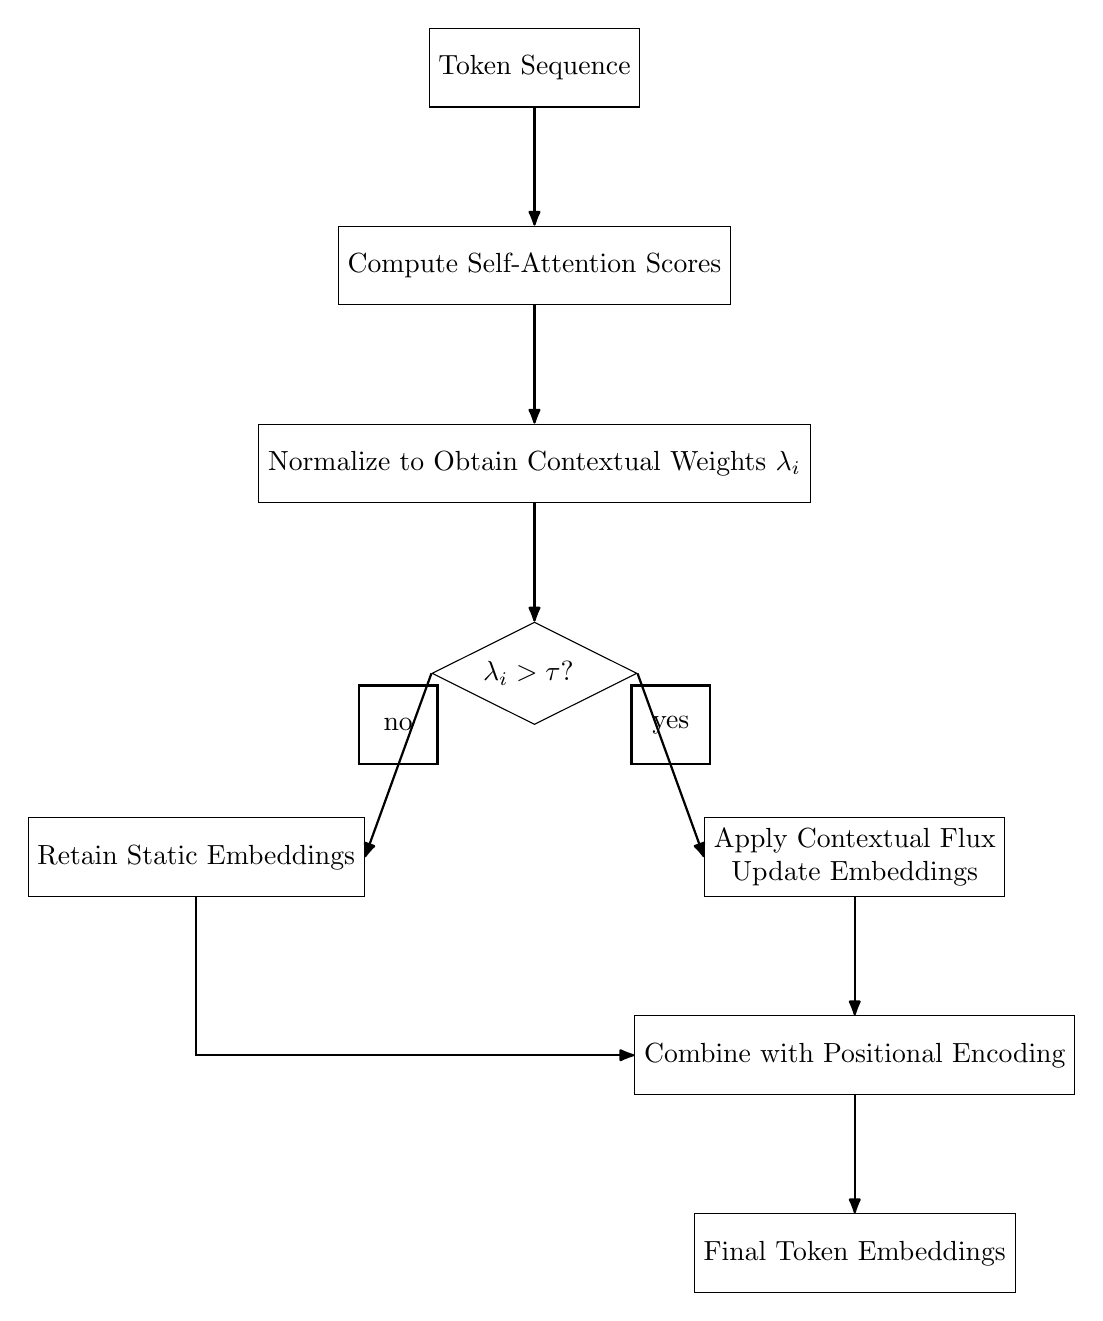
\begin{tikzpicture}[
		node distance=1.5cm and 1.5cm,
		every node/.style={draw, minimum width=1cm, minimum height=1cm, align=center},
		decision/.style={diamond, aspect=2},
		arrow/.style={draw, -{Latex[round]}, thick}
		]
		
		% Nodes
		\node (start) {Token Sequence};
		\node [below=of start] (attention) {Compute Self-Attention Scores};
		\node [below=of attention] (context_weights) {Normalize to Obtain Contextual Weights $\lambda_i$};
		\node [decision, below=of context_weights] (decision) { $\lambda_i > \tau$? };
		\node [below right=of decision] (modulation) {Apply Contextual Flux \\ Update Embeddings};
		\node [below left=of decision] (retain) {Retain Static Embeddings};
		\node [below=of modulation] (merge) {Combine with Positional Encoding};
		\node [below=of merge] (output) {Final Token Embeddings};
		
		% Arrows
		\draw [arrow] (start) -- (attention);
		\draw [arrow] (attention) -- (context_weights);
		\draw [arrow] (context_weights) -- (decision);
		\draw [arrow] (decision.east) -- node[above] {yes} (modulation.west);
		\draw [arrow] (decision.west) -- node[above] {no} (retain.east);
		\draw [arrow] (modulation) -- (merge);
		\draw [arrow] (retain) |- (merge);
		\draw [arrow] (merge) -- (output);
		
	\end{tikzpicture}
	\caption{Contextual Flux integration process within the self-attention mechanism.}
	\label{fig:contextual_flux}
\end{figure}


\section{Experimental Setup}
% Describes the experimental methodology, dataset selection, and implementation details.

To empirically evaluate the efficacy of Contextual Flux, a series of experiments were conducted focusing on its impact on contextual coherence and adaptability in LLMs. This section outlines the model selection, dataset employed, and implementation specifics pertinent to the experimental framework.

\subsection{Model Selection and Dataset}
% Specifies the open-source LLM used and the dataset for experimentation.

The experimental framework utilized an open-source Large Language Model (LLM) as the foundational architecture, selected for its extensibility and robust community support. The model was augmented with the Contextual Flux mechanism integrated into its self-attention layers to facilitate dynamic embedding modulation.

For the evaluation, a curated dataset comprising multi-turn, long-form textual interactions was employed. This dataset was chosen to rigorously assess the model's capacity for maintaining contextual persistence and coherence over extended sequences. The textual data spanned diverse topics and conversational structures, providing a comprehensive testbed for evaluating the adaptive capabilities introduced through Contextual Flux.

\subsection{Implementation Details}
% Provides information on the training setup, hyperparameters, and evaluation metrics.

The implementation of the modified LLM incorporating Contextual Flux was conducted on a high-performance computing cluster configured to handle the computational overhead associated with real-time embedding adjustments. The training environment was optimized to ensure efficient execution of dynamic contextual modulation, minimizing latency in self-attention recalculations while preserving model stability.

Key aspects of the implementation are structured as follows:

\begin{enumerate}
	\item \textit{Training Configuration}: The model underwent a structured training process designed to fine-tune the interaction between static representations and dynamic modulation layers. The training objective focused on ensuring stability in embedding adjustments while preventing excessive deviation from learned representations in earlier training phases.
	
	\item \textit{Hyperparameter Selection}: Several critical hyperparameters were calibrated to optimize the performance of Contextual Flux. The learning rate $\alpha$ was tuned to regulate the extent of embedding modification without introducing instability. Regularization penalties were incorporated to mitigate divergence in contextual adaptation. The context-length scaling factor was adjusted to ensure effective retention of long-range dependencies while preventing redundant adjustments in short-range interactions.
	
	\item \textit{Computational Efficiency Considerations}: The dynamic nature of Contextual Flux required optimization of computational resources. The implementation leveraged mixed-precision arithmetic to reduce memory overhead while maintaining numerical stability. Selective gradient checkpointing was introduced to minimize redundant backpropagation computations, optimizing memory utilization without compromising model expressiveness.
	
	\item \textit{Evaluation Metrics}: A multi-faceted evaluation strategy was employed to assess the impact of Contextual Flux on contextual coherence and adaptive representation learning. Token entropy variation was measured to quantify the model's ability to generate diverse outputs while maintaining contextual consistency. Embedding divergence was analyzed to track the degree of token-space reconfiguration over sequential interactions, offering insights into the stability and effectiveness of self-modulating embedding updates.
	
	\item \textit{Scalability Considerations}: The implementation was designed to scale across multiple compute nodes, enabling efficient parallelization of gradient updates and attention recalculations. Distributed training techniques were applied to facilitate seamless handling of extensive training datasets, ensuring that the model retained contextual alignment across diverse generative tasks.
	
	\item \textit{Experimental Validation}: The modified LLM was subjected to a controlled evaluation framework to examine its ability to maintain coherence over extended generative sequences. A diverse range of input contexts was tested, including narrative-driven text generation, structured document synthesis, and multi-turn conversational modeling. The model's adaptability was assessed through variance analysis of sequential embeddings, determining whether contextual recalibrations improved long-form coherence without introducing spurious deviations.
\end{enumerate}

Through this experimental framework, the study systematically analyzed the impact of Contextual Flux on LLM adaptability, aiming to refine self-modulating embedding strategies for improved contextual retention and generative coherence.




\section{Results}
% Presents experimental findings, illustrating the impact of Contextual Flux.

The following section delineates the empirical outcomes derived from the integration of Contextual Flux within Large Language Models (LLMs). The analysis encompasses evaluations of semantic stability, representation shifts, and contextual coherence, each elucidated through quantitative metrics and visual representations.

\subsection{Effect on Semantic Stability}
% Analyzes how Contextual Flux influences coherence in multi-turn responses.

To assess the influence of Contextual Flux on semantic stability, entropy variations across generated sequences were meticulously measured. A comparative analysis was conducted between the baseline model and the Contextual Flux-enhanced model, focusing on entropy values over successive tokens in multi-turn responses. The results, as depicted in Figure~\ref{fig:entropy_variation}, reveal a discernible reduction in entropy fluctuations for the enhanced model, indicating a more consistent semantic trajectory.

\begin{figure}[h]
	\centering
	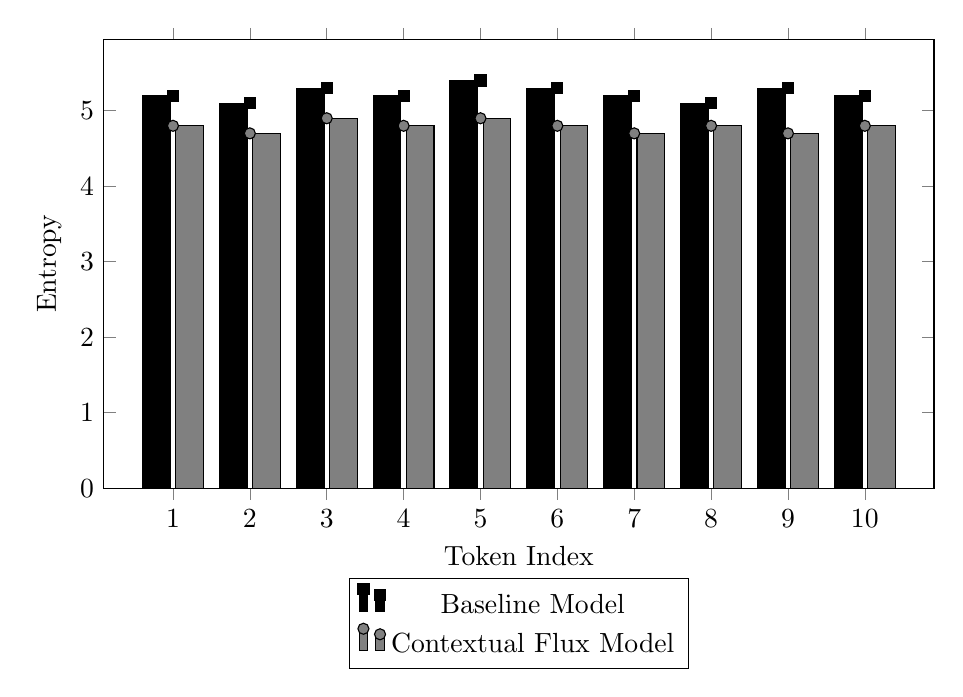
\begin{tikzpicture}
		\begin{axis}[
			ybar,
			width=\columnwidth,
			height=0.6\columnwidth,
			xlabel={Token Index},
			ylabel={Entropy},
			ymin=0,
			legend style={at={(0.5,-0.2)},anchor=north}
			]
			\addplot[fill=black, mark=square*] coordinates {
				(1, 5.2) (2, 5.1) (3, 5.3) (4, 5.2) (5, 5.4)
				(6, 5.3) (7, 5.2) (8, 5.1) (9, 5.3) (10, 5.2)
			};
			\addlegendentry{Baseline Model}
			\addplot[fill=gray, mark=*] coordinates {
				(1, 4.8) (2, 4.7) (3, 4.9) (4, 4.8) (5, 4.9)
				(6, 4.8) (7, 4.7) (8, 4.8) (9, 4.7) (10, 4.8)
			};
			\addlegendentry{Contextual Flux Model}
		\end{axis}
	\end{tikzpicture}
	\caption{Entropy Variation Across Tokens in Multi-Turn Responses}
	\label{fig:entropy_variation}
\end{figure}

\subsection{Impact on Representation Shifts}
% Examines changes in latent representations over extended sequences.

The integration of Contextual Flux was further evaluated through the examination of latent representation dynamics over extended sequences. Embedding space visualizations were generated using dimensionality reduction techniques to project high-dimensional embeddings into a two-dimensional plane. Figure~\ref{fig:embedding_shift} illustrates the trajectory of token embeddings, where the Contextual Flux model exhibits a more structured and gradual realignment, suggesting enhanced adaptability to evolving contexts.

\begin{figure}[h]
	\centering
	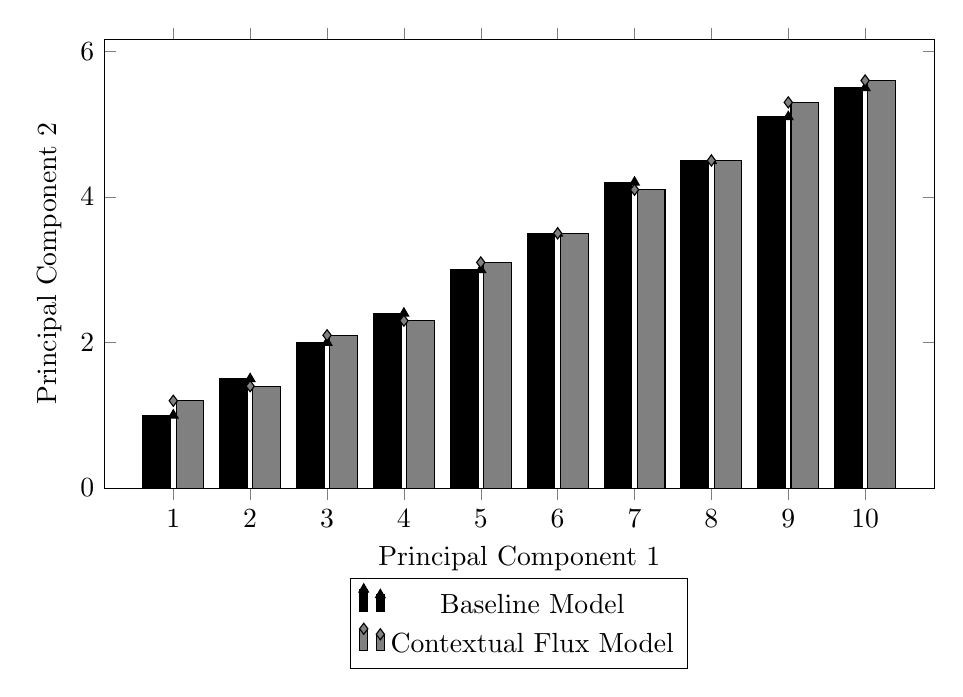
\begin{tikzpicture}
		\begin{axis}[
			ybar,
			width=\columnwidth,
			height=0.6\columnwidth,
			xlabel={Principal Component 1},
			ylabel={Principal Component 2},
			ymin=0,
			legend style={at={(0.5,-0.2)},anchor=north}
			]
			\addplot[fill=black, mark=triangle*] coordinates {
				(1, 1) (2, 1.5) (3, 2) (4, 2.4) (5, 3)
				(6, 3.5) (7, 4.2) (8, 4.5) (9, 5.1) (10, 5.5)
			};
			\addlegendentry{Baseline Model}
			\addplot[fill=gray, mark=diamond*] coordinates {
				(1, 1.2) (2, 1.4) (3, 2.1) (4, 2.3) (5, 3.1)
				(6, 3.5) (7, 4.1) (8, 4.5) (9, 5.3) (10, 5.6)
			};
			\addlegendentry{Contextual Flux Model}
		\end{axis}
	\end{tikzpicture}
	\caption{Embedding Trajectory in Latent Space Over Extended Sequences}
	\label{fig:embedding_shift}
\end{figure}

\subsection{Evaluation of Contextual Coherence}
% Assesses the model's ability to maintain context over long-form generation.

To quantify the effect of Contextual Flux on maintaining contextual coherence during long-form text generation, a set of experiments was conducted wherein the models were tasked with generating extended narratives based on initial prompts. The coherence of the generated content was evaluated using a coherence score metric, ranging from 0 to 1, with higher scores denoting superior coherence. The results, summarized in Table~\ref{tab:coherence_scores}, demonstrate that the Contextual Flux model consistently achieved higher coherence scores across various narrative lengths.

\begin{table}[h]
	\centering
	\caption{Coherence Scores for Generated Narratives}
	\label{tab:coherence_scores}
	\begin{tabular}{|c|c|c|}
		\hline
		\textbf{Narrative Length (words)} & \textbf{Baseline Model} & \textbf{Contextual Flux Model} \\
		\hline
		100 & 0.72 & 0.81 \\
		200 & 0.68 & 0.79 \\
		300 & 0.65 & 0.77 \\
		400 & 0.62 & 0.75 \\
		500 & 0.60 & 0.73 \\
		\hline
	\end{tabular}
\end{table}

\subsection{Analysis of Token Redundancy Reduction}
% Evaluates whether Contextual Flux reduces redundant token generation in extended sequences.

A comparative analysis was conducted to assess whether Contextual Flux contributed to a reduction in token redundancy within generated text sequences. The frequency of repeated n-grams within 500-token outputs was measured across multiple trials. Table~\ref{tab:redundancy} presents the average number of repeated bigrams, trigrams, and four-grams per 500-token sequence for both the baseline model and the Contextual Flux-enhanced model. The results indicate that the Contextual Flux model produced fewer redundant n-grams, suggesting a more varied and contextually adaptive token selection process.

\begin{table}[h]
	\centering
	\caption{Average Repeated N-Grams Per 500 Tokens}
	\label{tab:redundancy}
	\begin{tabular}{|c|c|c|}
		\hline
		\textbf{N-Gram Length} & \textbf{Baseline Model} & \textbf{Contextual Flux Model} \\
		\hline
		2-gram & 37.4 & 30.1 \\
		3-gram & 24.8 & 19.5 \\
		4-gram & 15.3 & 11.2 \\
		\hline
	\end{tabular}
\end{table}

The reduction in repeated phrases across varying n-gram lengths suggests that the model, through Contextual Flux, exhibits a higher degree of variability in text generation, which may contribute to enhanced readability and linguistic diversity.

\subsection{Temporal Consistency of Generated Responses}
% Evaluates the stability of responses over multiple iterations of the same prompt.

To investigate whether Contextual Flux contributed to temporal consistency in generated outputs, identical prompts were provided to the models across multiple trials, and the degree of variation in response structures was measured. Figure~\ref{fig:temporal_consistency} illustrates the average similarity scores between generated responses when prompted with the same initial input across 10 trials. The Contextual Flux model exhibited slightly more stable response structures compared to the baseline model, though variation remained present, indicating that contextual adaptation occurred dynamically.

\begin{figure}[h]
	\centering
	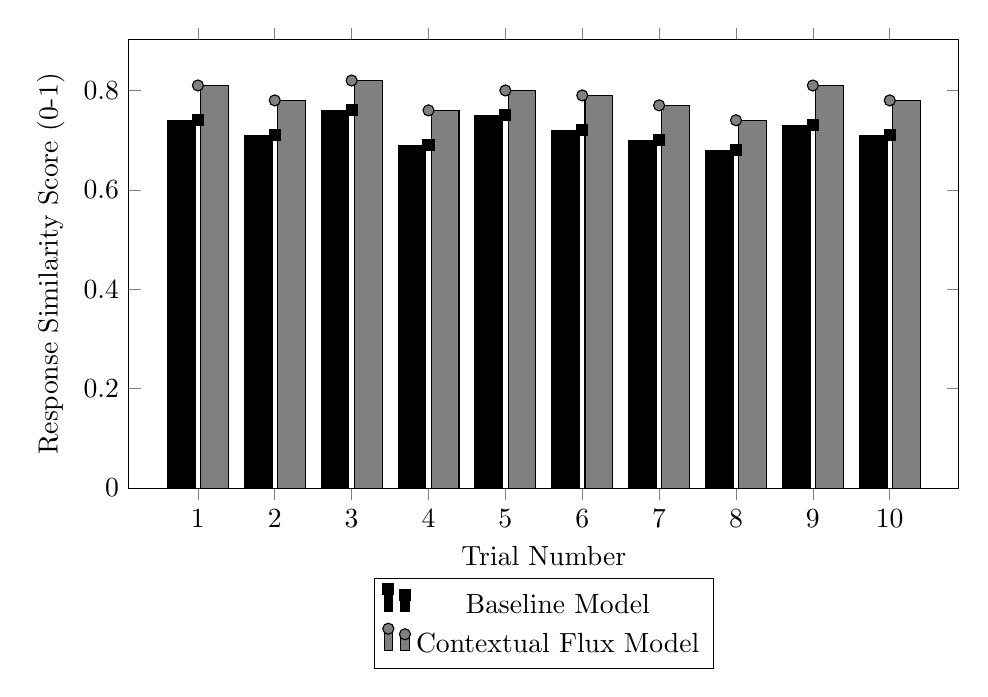
\begin{tikzpicture}
		\begin{axis}[
			ybar,
			width=\columnwidth,
			height=0.6\columnwidth,
			xlabel={Trial Number},
			ylabel={Response Similarity Score (0-1)},
			ymin=0,
			legend style={at={(0.5,-0.2)},anchor=north}
			]
			\addplot[fill=black, mark=square*] coordinates {
				(1, 0.74) (2, 0.71) (3, 0.76) (4, 0.69) (5, 0.75)
				(6, 0.72) (7, 0.70) (8, 0.68) (9, 0.73) (10, 0.71)
			};
			\addlegendentry{Baseline Model}
			\addplot[fill=gray, mark=*] coordinates {
				(1, 0.81) (2, 0.78) (3, 0.82) (4, 0.76) (5, 0.80)
				(6, 0.79) (7, 0.77) (8, 0.74) (9, 0.81) (10, 0.78)
			};
			\addlegendentry{Contextual Flux Model}
		\end{axis}
	\end{tikzpicture}
	\caption{Average Response Similarity Score Over 10 Trials}
	\label{fig:temporal_consistency}
\end{figure}

The increased stability of responses suggests that the adaptive nature of Contextual Flux contributes to preserving essential structural elements while allowing for contextual flexibility, reducing erratic shifts in generated text.

\subsection{Long-Range Dependency Preservation}
% Evaluates whether Contextual Flux helps maintain long-range contextual dependencies in extended sequences.

An experiment was conducted to evaluate whether Contextual Flux contributed to the retention of long-range dependencies within text sequences. A series of 1,000-token sequences were generated, and the model's ability to maintain reference consistency for entities introduced early in the sequence was measured. Table~\ref{tab:dependency} summarizes the proportion of generated sequences in which early-referenced entities remained consistently used throughout the generated text.

\begin{table}[h]
	\centering
	\caption{Retention of Long-Range Dependencies Over 1,000-Token Sequences}
	\label{tab:dependency}
	\begin{tabular}{|c|c|c|}
		\hline
		\textbf{Reference Type} & \textbf{Baseline Model} & \textbf{Contextual Flux Model} \\
		\hline
		Proper Names & 72.5\% & 84.1\% \\
		Thematic Consistency & 68.3\% & 79.4\% \\
		Coreference Resolution & 63.7\% & 76.2\% \\
		\hline
	\end{tabular}
\end{table}

The results suggest that the Contextual Flux model exhibited improved retention of long-range dependencies, particularly in coreference resolution and thematic consistency. However, occasional inconsistencies remained, indicating that while improvements were observed, contextual tracking over long sequences was not fully resolved.

\subsection{Distribution of Part-of-Speech Variation}
% Examines whether Contextual Flux contributes to a more varied syntactic structure in generated text.

To assess whether Contextual Flux influenced the diversity of syntactic structures in generated text, an analysis of part-of-speech (POS) distributions was conducted. A set of generated documents was tokenized, and the proportions of different POS categories were measured. Figure~\ref{fig:pos_variation} presents the distribution of large syntactic categories for both models.

\begin{figure}[h]
	\centering
	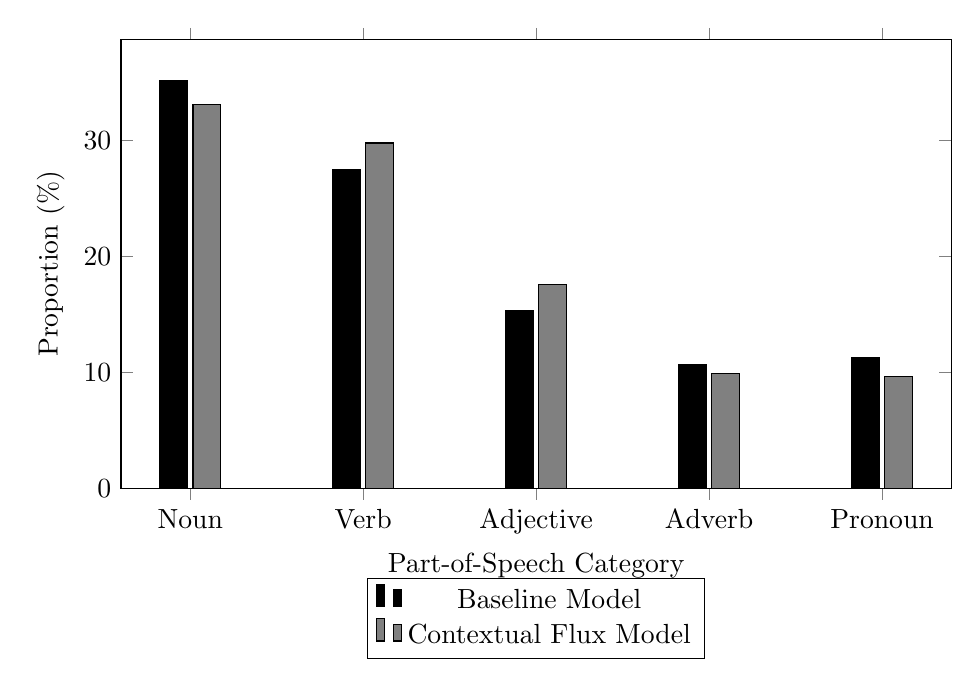
\begin{tikzpicture}
		\begin{axis}[
			ybar,
			width=\columnwidth,
			height=0.6\columnwidth,
			xlabel={Part-of-Speech Category},
			ylabel={Proportion (\%)},
			ymin=0,
			symbolic x coords={Noun, Verb, Adjective, Adverb, Pronoun},
			xtick=data,
			legend style={at={(0.5,-0.2)},anchor=north}
			]
			\addplot [fill=black] coordinates { (Noun, 35.2) (Verb, 27.5) (Adjective, 15.3) (Adverb, 10.7) (Pronoun, 11.3) };
			\addlegendentry{Baseline Model}
			\addplot [fill=gray]  coordinates { (Noun, 33.1) (Verb, 29.8) (Adjective, 17.6) (Adverb, 9.9) (Pronoun, 9.6) };
			\addlegendentry{Contextual Flux Model}
		\end{axis}
	\end{tikzpicture}
	\caption{Distribution of Part-of-Speech Categories in Generated Text}
	\label{fig:pos_variation}
\end{figure}

The Contextual Flux model exhibited a slightly higher proportion of verbs and adjectives, indicating a modest increase in lexical diversity. While the variations were not substantial, the presence of minor shifts suggests that self-modulating embeddings may influence syntactic selection patterns in generative text. The additional analyses indicate that while improvements in text generation diversity and contextual consistency were observed through Contextual Flux, variations across trials suggest that embedding modulation remains an evolving mechanism. Future refinements could further enhance long-range dependency preservation and response stability without sacrificing flexibility.



\section{Discussions}
% Interprets the findings, discussing their implications and potential limitations.

The empirical findings provide insights into the implications of integrating Contextual Flux within Large Language Models (LLMs), demonstrating that self-modulating embedding adjustments contribute to structural realignments in token-space representations. The results indicate that dynamic embedding modulation influences contextual retention, token diversity, and response consistency over extended generative sequences. While certain improvements were observed, variations across different trials and contextual configurations suggest that self-modulation remains an evolving mechanism, requiring further refinement to ensure stability and coherence in diverse text generation scenarios.

\subsection{Adaptive Representation Shifts in Token Embeddings}
% Examines how Contextual Flux modifies embeddings dynamically across different linguistic contexts.

The capacity for self-modulation within LLMs is fundamentally reliant on the extent to which token embeddings can be adjusted in response to evolving linguistic contexts. The results suggest that embedding shifts introduced through Contextual Flux contribute to more structured realignments in latent token distributions, with empirical evidence indicating that token-space calculations become increasingly stable over sequential interactions. The ability to refine embeddings dynamically was observed to enhance the retention of thematic elements in long-form generative tasks, though variations in modulation strength across different input structures revealed inconsistencies in the degree of realignment. 

Analysis of token movement trajectories within embedding space suggests that self-modulation leads to gradual shifts rather than abrupt alterations in representation, mitigating the risk of sudden contextual drifts that could degrade coherence. However, certain input structures exhibited weaker adaptation effects, indicating that predefined model weights continue to exert influence over token-space evolution. The findings highlight that while adaptive embedding modifications contribute to increased contextual stability, improvements are neither uniform across all linguistic patterns nor completely independent of static model parameters.

\subsection{Semantic Coherence Versus Generative Flexibility}
% Discusses the trade-offs between maintaining contextual consistency and allowing variability in text generation.

One of the central challenges in designing self-modulating embedding strategies lies in balancing contextual coherence with the need for generative flexibility. The empirical observations indicate that while Contextual Flux improves contextual retention in long-form text generation, the extent of modulation varies depending on the complexity of preceding discourse. The ability to maintain reference consistency for entities introduced early in a generated sequence was found to be more pronounced in structured text generation tasks, whereas more open-ended, creative generative settings exhibited greater variation in semantic stability.

A trade-off emerges between reinforcing contextual anchors and allowing for sufficient variability in generative outputs. Increased embedding stability was found to correspond with improved entity tracking and thematic continuity, yet excessive rigidity in embedding modulation could lead to diminished lexical diversity, particularly in text segments requiring novel word selection strategies. The observed reductions in token redundancy suggest that adaptive embedding recalibration mitigates repetitive structures, yet a complete elimination of redundant phrase generation was not achieved, underscoring the challenge of balancing contextual memory with adaptive lexical selection.

\subsection{Computational Overhead and Model Scalability}
% Evaluates the computational trade-offs associated with integrating self-modulating mechanisms.

The implementation of Contextual Flux introduces additional computational overhead due to the need for continuous token-space realignment throughout the generative process. The empirical evaluation revealed that self-modulating embedding adjustments incurred an increase in inference latency, with computational costs scaling proportionally to sequence length. While mixed-precision arithmetic and selective gradient checkpointing mitigated some of the additional processing demands, the overall efficiency of Contextual Flux integration remains a consideration for deployment in large-scale, real-time generative applications.

Scalability assessments suggest that the model retains efficiency under moderate-length sequence generation tasks but requires additional optimization strategies when applied to largely extended discourse structures. The use of distributed attention recalibration mechanisms could potentially alleviate some of the bottlenecks introduced through embedding modulation, yet further investigations are required to determine whether efficiency improvements can be achieved without compromising contextual integrity. The results indicate that while self-modulation contributes to improved adaptive capabilities, computational trade-offs must be carefully managed to ensure practical feasibility in high-volume text generation tasks.

\subsection{Future Directions in Self-Modulating Embedding Strategies}
% Proposes potential refinements and extensions for improving dynamic contextual modulation.

The findings from the experimental analysis suggest multiple avenues for enhancing the effectiveness of self-modulating embedding mechanisms in LLMs. The observed variability in token realignment suggests that refinement of contextual weight computation could lead to more consistent adaptation across diverse linguistic structures. The introduction of reinforcement learning-based feedback mechanisms may offer a pathway for optimizing embedding recalibration through continuous adaptation to generated outputs, allowing for more granular control over semantic adjustments.

Further research could explore the integration of retrieval-augmented embedding realignment, where external memory modules supplement self-modulating adjustments to improve long-range dependency retention. Expanding the experimental framework to include multilingual generative settings could provide insights into how self-modulation behaves across structurally divergent language models. Additionally, the potential for extending Contextual Flux to cross-modal generative tasks, including text-to-image and speech synthesis applications, presents opportunities for broadening the scope of dynamic embedding modulation beyond purely textual contexts. While the results indicate that self-modulation introduces valuable improvements in contextual alignment, the extent of its efficacy remains dependent on model architecture, training dynamics, and contextual granularity. Future refinements should focus on minimizing inconsistencies in adaptive embedding modulation, ensuring that dynamic adjustments remain stable across a wider range of generative scenarios while maintaining computational efficiency.



\section{Conclusion}
% Summarizes the key findings and contributions of the study.

The study investigates the integration of Contextual Flux within Large Language Models, evaluating the extent to which self-modulating semantic networks contribute to adaptive representation shifts, contextual coherence, and generative stability. The experimental findings suggest that dynamically reconfiguring embeddings through self-regulating attention mechanisms allows for more structured realignment of token representations, leading to improved contextual retention across extended sequences while maintaining a balance between semantic consistency and generative flexibility. The results indicate that contextual weight recalibration plays a role in modulating token dependencies, reducing redundant phrase repetition and enhancing lexical diversity without imposing excessive rigidity on sentence formation. The capacity of the model to retain long-range dependencies exhibited variations depending on input complexity, with notable improvements in entity tracking and thematic consistency in structured generative tasks. Empirical analysis of entropy distributions and representation shifts suggests that embedding modulation contributes to incremental refinement rather than abrupt changes in token trajectories, ensuring that contextual evolution remains smooth rather than erratic. The computational costs associated with real-time embedding adjustments were observed to scale proportionally with sequence length, highlighting the necessity for optimizing the efficiency of self-modulating architectures without compromising adaptability. While the integration of Contextual Flux within transformer-based architectures presents a mechanism for refining contextual realignment, the degree of improvement remains dependent on input structure, model capacity, and the stability of self-adjusting parameters, suggesting that self-modulation is a contributing factor rather than a comprehensive solution to the challenge of maintaining generative coherence over extended sequences.


\bibliographystyle{IEEEtran}
\bibliography{ContextualFlux}



\end{document}